% !TEX root = perelman-geometry.tex
%!TEX TS-program = pdflatex
%!TEX encoding = UTF-8 Unicode


\maketitle
\cleardoublepage
\thispagestyle{empty}
%\pagenumbering{roman}
\begin{center}

{\LARGE Ya. I. Perelman}

{\Huge Geometry for Entertainment}




The Mir Titles Project

\end{center}
\cleardoublepage

\thispagestyle{empty}
\vfill
\begin{small}

{\noindent
Seventh Edition, Revised

Edited and supplemented by \emph{B.A. Kordemsky}

First Published by State Publishing House Of Technical And Theoretical Literature Moscow -- 1950 -- Leningrad.

Original scan in Russian by the \emph{Russian Lutherean}\\ \url{https://archive.org/details/20220910_perelman_geometry/}.

Translated from the Russian and typeset in \LaTeX{} using Linux Libertine by \emph{Damitr Mazanav}.

This fully electronic English translation released in 2024 by \\\textsc{the mir titles project} \url{https://mirtitles.org} .

Source files available at \\ \url{https://gitlab.com/mirtitles/perelman-geometry}
 
Front cover: Woodcut from Cosimo Bartoli's \emph{Del modo di misvrare} published in 1564. \\ \url{https://archive.org/details/cosimobartolidel00bart}.

\copyright \emph{Damitr Mazanav}

Licence Creative Commons by NC 4.0}


\includegraphics[width=0.3\textwidth]{figures/cc-by-nc.pdf}

\end{small}

\cleardoublepage

 \tableofcontents
 
 \cleardoublepage

\chapter{Editor's Preface}
\label{editor-preface}
%\addcontentsline{toc}{chapter}{\nameref{preface}}


\emph{Geometry for Entertainment} is written both for friends of mathematics and for those readers from whom many attractive aspects of mathematics have somehow been hidden.

More importantly, this book is intended for those readers who studied (or are currently studying) geometry only at the blackboard and therefore are not used to noticing familiar geometric relationships in the world of things and phenomena around us, have not learnt to use the acquired geometric knowledge in practise, in difficult cases of life, on a hike, in a bivouac or front-line situation.

To arouse the reader's interest in geometry or, in the words of the author, ``to inspire a desire and cultivate a taste for its study is the objective of this book.''

To this end, the author will take geometry ``out of the walls of the school room into the free air, into the forest, field, to the river, on the road, in order to indulge in relaxed geometric studies without a textbook and tables in the open air \ldots{}'', and draws the reader's attention to the pages of L. N. Tolstoy and A. P. Chekhov, Jules Verne and Mark Twain. He finds a theme for geometric problems in the works of N. V. Gogol and A. S. Pushkin, and finally offers the reader ``a motley selection of problems, curious in plot, unexpected in result.''

The seventh edition of \emph{Geometry for Entertainment} is published without the direct participation of the author. Ya. I. Perelman died in Leningrad in 1942.

The new edition of the book contains almost all the articles of the previous edition, newly illustrated, edited and supplemented with facts and information from our Soviet reality, as well as a considerable number (about 30) additional articles.

I was guided by the desire to increase the ``utility coefficient'' of Ya. Perelman's book, to make it even more effective and interesting, involving new readers in the ranks of friends of mathematics.

To what extent this was possible, I hope to learn from readers at the address: Moscow, 64, Chernyshevsky Str., 81, Sq. 53, B. A. Kordemsky.


\begin{flushright}
\emph{B. Kordemsky}
\end{flushright}


\chapter{Translator's Preface}
\label{translator-preface}
%\addcontentsline{toc}{chapter}{\nameref{preface}}

Yakov Perelman's books have been a constant source of inspiration for me throughout my life. Though many of his works have been translated to English and other languages, several works remain untranslated. As a part of Mir Titles Project we endeavour to bring all such works to the people. This translation is a rather ambitious project and it brings me great pleasure to present this untranslated work of Perelman into an English version. 

\marginnote{Illustrations}The beautiful and abundant illustrations in the form of woodcuts, are the heart of the book. Geometry being primarily reliant on illustrations, is brought to life in a variety of situations. Familiar geometrical shapes, lines, ratios are found amongst trees, rivers, homes, skies and other natural settings. This makes everyday objects the familiarly mathematical. 

Each topic is complemented by relevant illustrations which make understanding them easier. Being woodcuts, it was easy for me to convert them to digital form. I have made no effort to change the images, except in some cases replacing the Russian letters with Roman ones.


\marginnote{Examples}In his discussions emphasises the geometrical relationships in the measurable and unknown quantities. This approach is historical in the sense that this is how geometry developed: to solve problems of measurement of unknown quantities. Thus we have problems related to measuring a variety of things, using direct measurement or very primitive instruments. 



\marginnote{Translation}I have made use of machine translations for the bulk of text, and it has worked at a satisfactory level. At times I have made use of several translation services to make sure I am on right track and the meaning is not lost in translation. 

\marginnote{Typesetting}During the course of typesetting this book, discussions posted on and help from kind people \LaTeX{} forum at stackexchange has been of great help. I have typeset the book in a square profile with marginpar for smaller figures and notes. 

If there are any mistakes in the mathematics or translation they are all mine. Any suggestions and criticisms to improve the translation are welcome. I hope that this English version finds enthusiastic readers and inspires many more brilliant minds in the generations to come.

\begin{flushright}
\emph{Damitr Mazanav}\\[5pt]
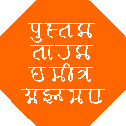
\includegraphics[width=0.2\textwidth]{figures/pustaktarak.pdf}
\end{flushright}
